Since the project was done as a double-period course at \LTU, $\SI{400}{\hour}$ per person was planned for the project over four months, this would amount to $400\cdot15=\SI{6000}{\hour}$ in total. To plan these hours, an agile workflow was adopted by dividing the work into sprints, where the end of each sprint represented a project presentation.

For each presentation, some new features were to be displayed, so goals representing those features were made up at the very start of the sprint and added to the taskboard. The developers then visited the taskboard to assign themselves some tasks that they believed they could handle and started working on it.

For instance, in the first presentation the architecture was to be presented and a simpler technical demonstration was planned. So, a proof-of-concept wherein python code was to be tested using a very simple user interface was designed. The idea was to include some mock data from the backend as well, but at the day of the presentation, the API was not yet ready. Therefore, right after the presentation, a new sprint goal to have the database setup and storing the progress of the corrected tests was planned for the next week.

\subsection{Taiga Sprint Planner}
Sprint planning was done using the open-source \taiga{} taskboard. By using a web-based tool, most planning could be done remotely instead of on a physical whiteboard. An idea was that it would allow participants to do their work remotely and not have to bother with visiting the project room. Taiga was chosen because it offered a free and gratis environment with little hassle for public projects, which seemed like a good fit for this project since everyone was eager to get started.

\begin{figure}[hb]
    \begin{subfigure}{.3\textwidth}
        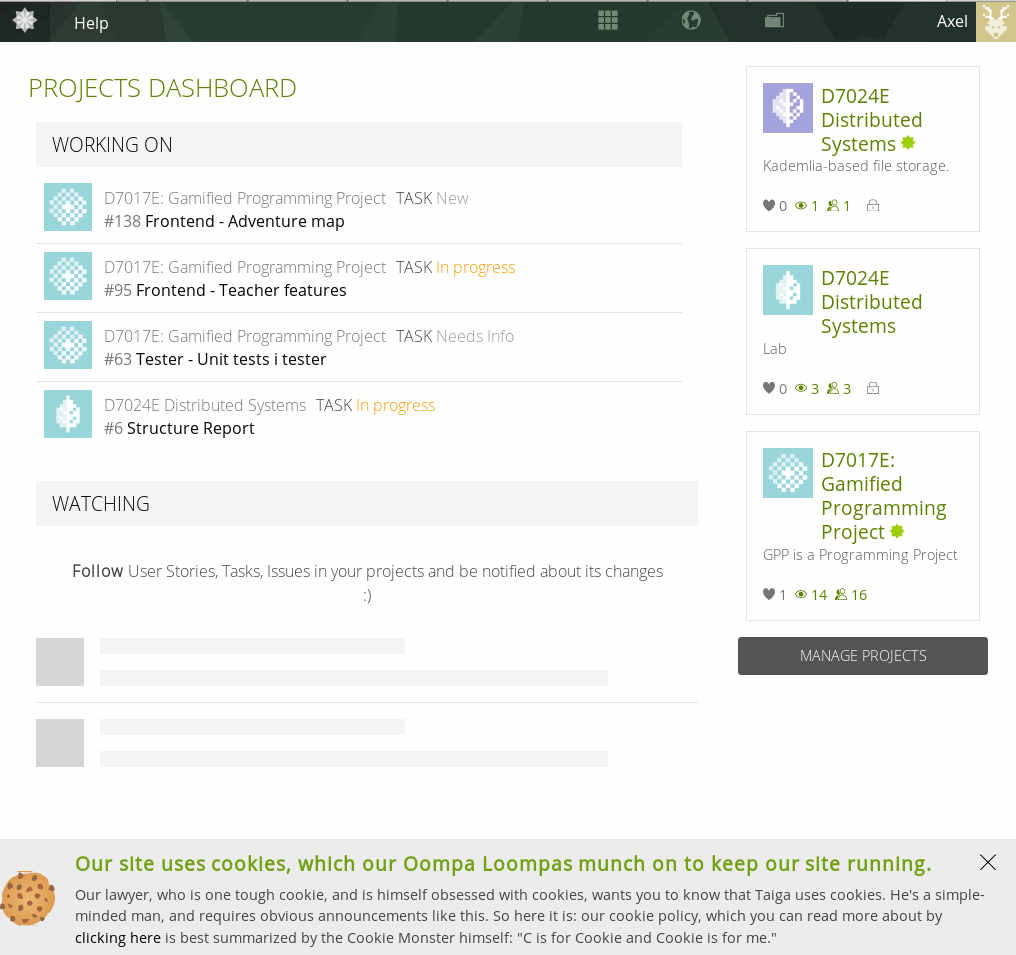
\includegraphics[width=\textwidth]{img/taiga_dash.jpg}
        \caption{Main dashboard}
    \end{subfigure}
    \hfill
    \begin{subfigure}{.3\textwidth}
        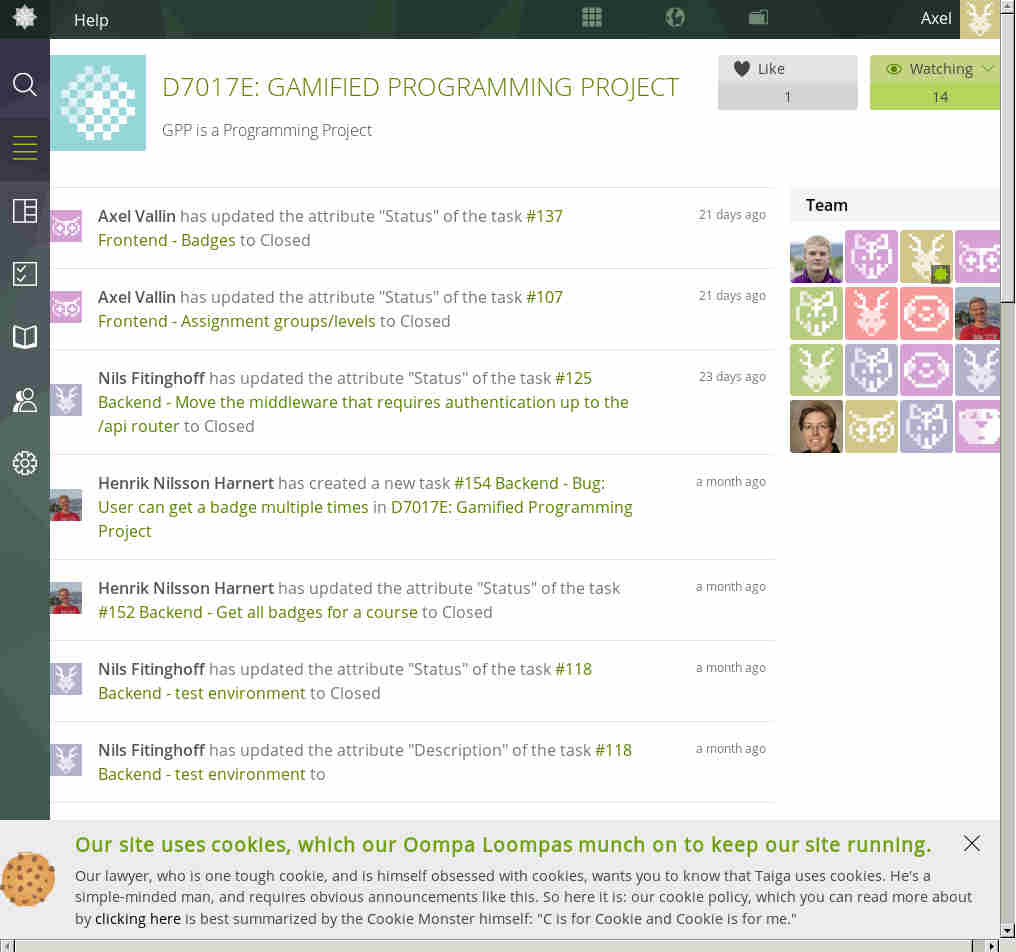
\includegraphics[width=\textwidth]{img/taiga_overview.jpg}
        \caption{Overview}
    \end{subfigure}
    \hfill
    \begin{subfigure}{.3\textwidth}
        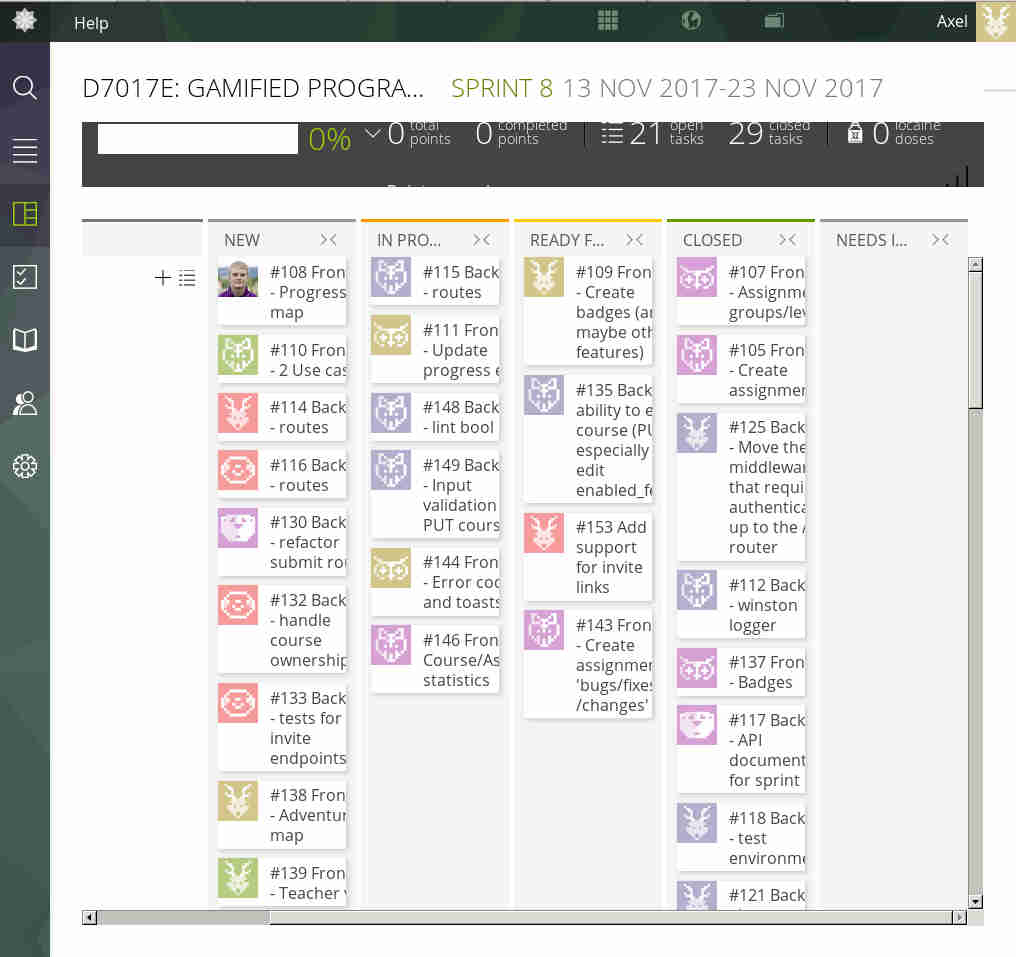
\includegraphics[width=\textwidth]{img/taiga_taskboard.jpg}
        \caption{Taskboard}
    \end{subfigure}
    \caption{Some screenshots from \taiga{}.}
\end{figure}

%Apart from \taiga{}, Trello was evaluated, but deemed too simple for a project of this size, furthermore some pay-to-use tools such as TODO: was looked at, but nobody wanted to pay for the service.
